
\chapter{A Ruler, a Broadcast, \& an Error Budget}
\label{sec:intro}

\noindent\emph{This section is deliberately pedagogical. It assumes no radio astronomy, no cosmology, and no detection theory, and it exists so that a reader from outside every one of those fields can follow the argument of the whole dissertation before meeting any of its mathematics. Later chapters distinguish what is specified by a standard, what is proved under an analytic model, what is measured from the archive, and what remains conditional on a calibration transfer. Figure~\ref{fig:intro:claimchain} gives that distinction a visual form at the outset.}

\begin{figure}[t]
\centering
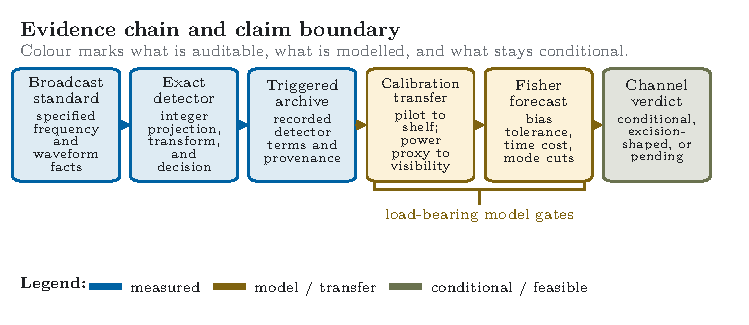
\includegraphics[width=0.98\linewidth]{figs/fig_claim_chain.pdf}
\caption[Evidence chain and claim boundary]{Evidence chain and claim boundary for the dissertation. The broadcast standard, exact detector, and recorded archive products are independently auditable. The transfers from a pilot statistic to the full DTV shelf, from a scalar power proxy to complex visibility residuals, and from a residual template to a cosmological verdict are model-dependent gates. Exact arithmetic secures the detector block; it does not by itself validate the scientific transfers downstream.}
\label{fig:intro:claimchain}
\end{figure}

\section{A Ruler Older Than the Stars}
\label{sec:intro:ruler}

Just after the Big Bang, the universe was a hot plasma of light and matter, so hot that atoms could not hold together. Light and matter were locked to each other --- photons scattering off free electrons, electrons bound by electric forces to the protons --- and the mixture behaved as a single fluid with enormous pressure. Wherever matter happened to be slightly overdense, gravity pulled inward and pressure pushed back out, and the contest launched sound waves: pressure waves in the plasma, physically the same phenomenon as sound in air, moving at more than half the speed of light. This much was worked out on paper decades before it was observed \cite{peebles1970,sunyaev1970}.

\begin{figure}[t]
\centering
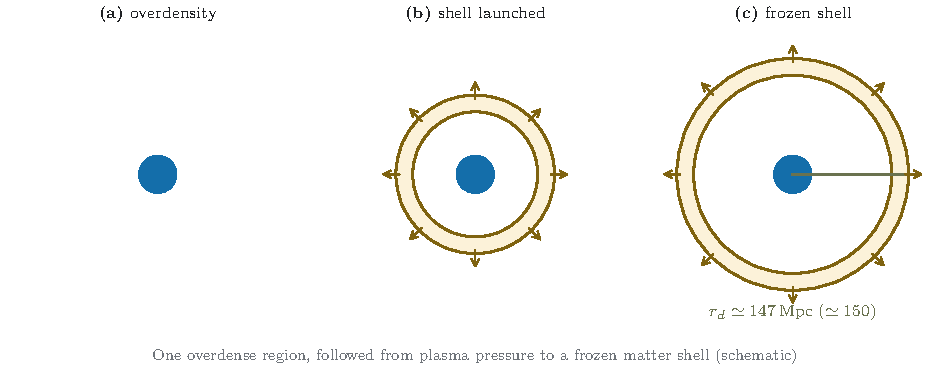
\includegraphics[width=0.98\linewidth]{figs/fig_intro_soundwave.pdf}
\caption{Where the ruler comes from (schematic). Follow one initially overdense spot. During the plasma era its pressure launches a spherical sound wave, which carries matter outward at over half the speed of light. When the universe cools enough for atoms to form --- about 380,000 years in --- the light that supplied the pressure escapes, the wave has nothing left to push it, and it simply stops where it is: a faint spherical shell of extra matter at the distance sound had traveled by that moment, the \emph{sound horizon} $s \approx 150$~Mpc. Every overdense spot in the universe did this simultaneously, so the pattern is imprinted statistically everywhere.}
\label{fig:intro:soundwave}
\end{figure}

Figure~\ref{fig:intro:soundwave} follows what happened next to a single overdense spot. Its sound wave spread outward as a growing spherical shell, carrying matter with it. Then, about 380,000 years after the Big Bang, the universe cooled through the temperature at which electrons and protons combine into neutral hydrogen. Recombination sharply reduced the free-electron density and therefore the Thomson opacity of the plasma, so the photons decoupled and streamed away --- we see them today as the cosmic microwave background --- and with them went the pressure that drove the wave. The shell stopped. It froze at exactly the distance sound had managed to travel in those 380,000 years: the \textbf{sound horizon}, about 150 megaparsecs once expanded to today's scale, roughly half a billion light-years. Every overdense region in the universe launched such a wave at the same time and froze it at the same radius, so the universe was left with a faint statistical preference for pairs of overdense regions separated by exactly that distance. Galaxies later formed where matter was dense --- both at the original centers and on the frozen shells --- and inherited the preference. It was detected directly in the distribution of half a million galaxies in 2005 \cite{eisenstein2005}, thirty-five years after it was predicted.

This is the baryon acoustic oscillation (BAO) scale, and it is the most trustworthy ruler cosmology owns. Its length is set by well-understood physics of the early universe --- the sound speed of a photon-baryon plasma and the age of the universe at recombination, both pinned tightly by the microwave background --- and by nothing that happened since. A ruler of known length is a way to measure distance: if the 150-Mpc separation \emph{appears} compressed or stretched at some epoch, that tells us exactly how much the universe expanded between that epoch and now. Measure the apparent size of the ruler at several epochs and the expansion history follows --- and the expansion history is where dark energy, whatever it is, shows itself.

The redshifts CHIME reaches are not an arbitrary stretch of that history. Somewhere around seven billion years ago the expansion of the universe stopped slowing down --- as gravity acting on matter says it must --- and began to speed up, which is the single observation the phrase ``dark energy'' exists to name. A ruler measurement made only nearby sees the acceleration but not the approach to it; a ruler measurement at $z \approx 1.3$--$2.0$, where CHIME's television-contested third of the band sits, watches the era when matter still governed the expansion and any departure from the simplest model of dark energy would first become visible. The transverse dilation at each redshift traces out the distance-redshift relation, the radial dilation traces the expansion rate itself, and together, epoch by epoch, they are the record dark-energy models must reproduce. This is why the redshifts under the television band are worth a dissertation-length fight: they are not spare bandwidth, they are the leverage arm of the whole measurement.

\section{The Wiggle}
\label{sec:intro:wiggle}

What does a ``statistical preference for one separation'' actually look like in data? Cosmologists compress a map of matter into a \textbf{correlation function}, written $\xi(r)$: the excess probability, relative to pure chance, that two regions separated by a distance $r$ are both overdense. If matter were scattered at random, $\xi$ would be zero at every separation. Gravity makes nearby regions strongly correlated, so $\xi$ is large at small $r$ and falls smoothly --- except at one special separation. At $r \approx 150$~Mpc the frozen shells contribute a small localized excess: the \textbf{bump} in the left panel of Figure~\ref{fig:intro:wiggle}. That bump \emph{is} the ruler, as it appears in a measurement.

\begin{figure}[t]
\centering
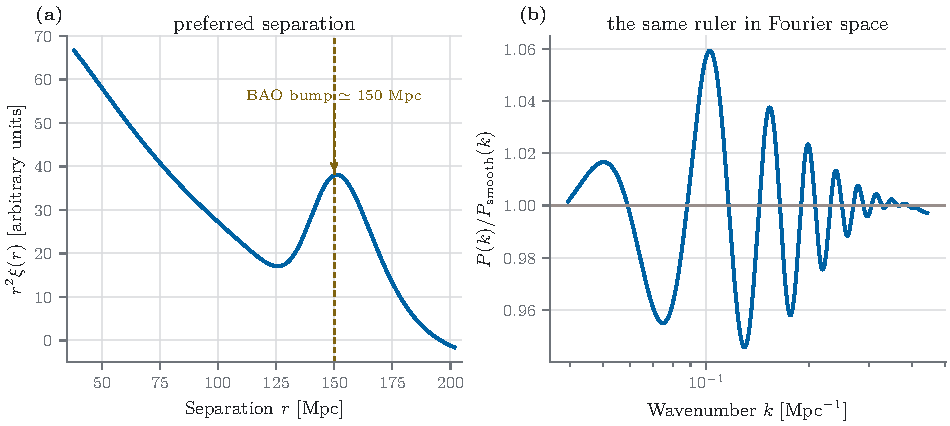
\includegraphics[width=0.98\linewidth]{figs/fig_intro_wiggle.pdf}
\caption{The ruler as it appears in data --- computed from the identical matter power spectrum used inside every forecast of Chapter~\ref{sec:bao} (CAMB, Planck-2018 fiducial). \emph{(a)} The correlation function: the excess tendency of two regions separated by $r$ to both be overdense, scaled by $r^2$ so the feature is visible against the smooth decline. The bump at 150~Mpc is the frozen shell of Figure~\ref{fig:intro:soundwave}, seen statistically. \emph{(b)} Exactly the same information organized by scale instead of separation: dividing the power spectrum $P(k)$ by a smooth, wiggle-free counterpart \cite{eisenstein1998} reveals the oscillations that give the phenomenon its name. A single preferred length produces a harmonic series, spaced $\Delta k = 2\pi/s$, damped toward small scales.}
\label{fig:intro:wiggle}
\end{figure}

The same information can be organized by scale instead of separation. Any map can be decomposed into waves of different wavelengths, and the \textbf{power spectrum} $P(k)$ records how much the map fluctuates at each wavenumber $k$ (long wavelengths at small $k$, short at large $k$). A single preferred separation in $\xi(r)$ becomes a series of \emph{oscillations} in $P(k)$ --- the right panel of Figure~\ref{fig:intro:wiggle} --- for the same reason a bell struck once rings with a fundamental and overtones: a feature localized at one scale in one description is a harmonic series in the other. These are the ``wiggles,'' and colloquially the whole feature is \emph{the wiggle}. The two descriptions are mathematically equivalent, and the forecast machinery of Chapter~\ref{sec:bao} works in $P(k)$; the intuition is often easier in $\xi(r)$, and this section will move between them freely. One more reason panel (b) is the operative picture: when Chapter~\ref{sec:bao} quotes a \emph{BAO detection significance}, the quantity being detected is precisely the amplitude of the curve in panel (b) --- the forecast writes $P(k) = P_{\rm smooth}(k)\,[1 + A\,f_{\rm BAO}(k)]$ with $f_{\rm BAO}$ the wiggle-only template, and ``detecting BAO'' means measuring $A$ away from zero, while the dilations are read from the \emph{phase} of the same oscillations. Detection reads the wiggle's amplitude; measurement reads where its nodes sit.

\begin{figure}[t]
\centering
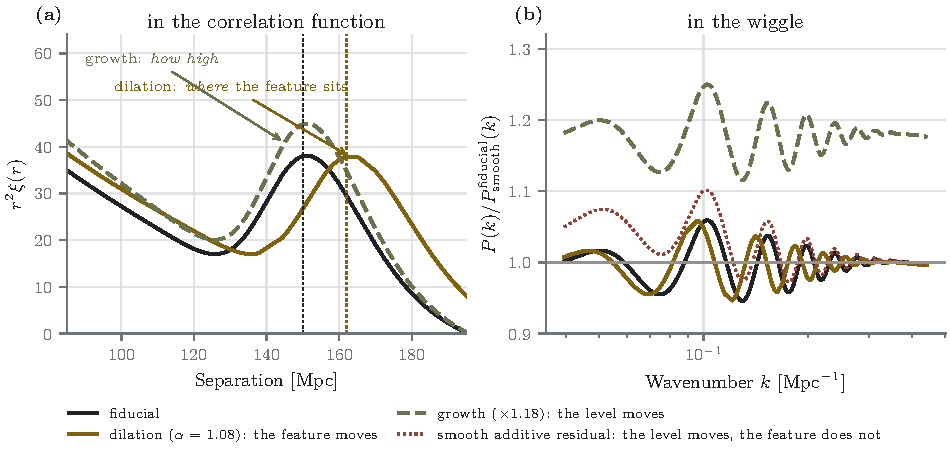
\includegraphics[width=0.98\linewidth]{figs/fig_intro_dilation.pdf}
\caption{Two ways to read the wiggle, drawn from the same forecast spectrum (offsets exaggerated for visibility). A \emph{dilation} slides the bump in separation without changing its shape: that is what the BAO parameters $\alpha_\perp$ and $\alpha_\parallel$ measure, and it is a geometry measurement --- where the feature sits. \emph{Growth} raises the whole curve where it stands: that is what $f\sigma_8$ measures, an amplitude. The distinction governs this dissertation's results: smoothly distributed contamination power mimics a change of amplitude far more readily than a shift of a feature's position, and Chapter~\ref{sec:bao} finds the measured tolerance for $f\sigma_8$ to be ten to twenty-five times tighter than for the dilations.}
\label{fig:intro:dilation}
\end{figure}

Three numbers are read off the wiggle, and Figure~\ref{fig:intro:dilation} shows what each one does to it. The first two ask \emph{where the bump sits}. Cosmologists predict its apparent position from a reference cosmology; the data are then fit for two \textbf{dilation} parameters, $\alpha_\perp$ and $\alpha_\parallel$, the ratios of the observed to the predicted position across and along the line of sight. (The two directions carry different information: across the sky the ruler's apparent size measures the distance to that epoch, while along the line of sight --- where distance is inferred from redshift --- it measures how fast the universe was expanding right then.) If the reference cosmology is right, both dilations come out 1.000; any departure is a discovery about the expansion history. These are \emph{feature-position} measurements, the BAO measurement proper.

The third number rides along in the same data. Galaxies are not merely carried by expansion; they also fall toward concentrations of matter, and those infall velocities add to the cosmological redshift. Along the line of sight, this compresses the apparent pattern by an amount proportional to how fast structure is growing \cite{kaiser1987} --- the phenomenon is called \textbf{redshift-space distortion}. Its strength is quoted as $f\sigma_8$: the growth rate $f$ times the overall clumpiness amplitude $\sigma_8$. Unlike the dilations, $f\sigma_8$ is an \emph{amplitude} measurement --- how strong the pattern is, not where its feature sits --- and that distinction, drawn in Figure~\ref{fig:intro:dilation}, turns out to govern the results of this dissertation. Contamination that adds smooth power to a map mimics a change of amplitude far more readily than it mimics a shift in a localized feature's position, so the growth rate will prove roughly an order of magnitude more fragile against interference than the ruler itself (Chapter~\ref{sec:bao}).

\section{Watching Hydrogen Instead of Galaxies}
\label{sec:intro:hydrogen}

The classical way to measure the wiggle is to catalog a few million galaxies, one by one, with their positions and redshifts. The Canadian Hydrogen Intensity Mapping Experiment (CHIME) takes a different route: it never resolves a single galaxy. Neutral hydrogen --- the most abundant element, present in and between galaxies everywhere --- emits at a precise radio wavelength of 21~cm (a frequency of 1420.4~MHz). Cosmic expansion stretches that emission in transit, by exactly the factor the universe expanded, so the frequency at which the line \emph{arrives} says how far back in time it \emph{departed}. A radio telescope tuned to one frequency is therefore looking at one definite slice of cosmic history. Frequency is distance. Tune across a band and you sweep out a three-dimensional volume, no catalog required.

This strategy is called \textbf{intensity mapping}: map the total 21~cm brightness in broad pixels --- each containing many unresolved galaxies --- and measure the statistical pattern, $\xi(r)$ or $P(k)$, directly from the map. The BAO-scale information is a property of that large-scale pattern and does not require resolving each galaxy, although intensity mapping carries its own tracer bias, calibration, foreground, and shot-noise limitations. What it gains is survey speed and volume. CHIME observes 400--800~MHz, which maps to redshifts $0.8 \le z \le 2.5$ --- light that left the hydrogen roughly seven to eleven billion years ago, spanning the approach to the epoch when the expansion of the universe stopped decelerating and began to accelerate \cite{amiri2022chime}. Modern spectroscopic surveys, especially DESI, now overlap much of this range with galaxies, quasars, and the Ly$\alpha$ forest \cite{desi2024iii,desi2024lya}; CHIME contributes a complementary tracer, enormous instantaneous volume, and a different set of systematics rather than an uncontested redshift domain.

The instrument itself matters to this dissertation's story, so one paragraph on it. CHIME is four fixed cylindrical reflectors, each 20~m by 100~m, like half-pipes laid side by side, with 1,024 dual-polarization receivers along their focal lines \cite{amiri2022chime}. It has no moving parts. It points nowhere, and therefore everywhere: the sky drifts overhead as the Earth turns, and the correlator reconstructs where each signal came from. Two consequences follow. First, enormous survey speed --- the whole northern sky, every day. Second, a property that will quietly become one of this work's main quantitative assets: an instrument that never points is differential in time, and emission fixed to the ground can project strongly onto modes removed by the sidereal analysis. Chapter~\ref{sec:bao} measures a 5--23~dB reduction in the scalar pilot-power proxy under a per-sidereal-day subtraction model. That reduction is useful, but it is not automatically identical to the attenuation of complex, baseline-dependent visibility contamination; the required transfer is made explicit there rather than treated as a free theorem.

The price of intensity mapping is faintness and foregrounds. The cosmological signal is of order a tenth of a millikelvin against a system temperature of tens of kelvin --- parts in a hundred thousand --- so the measurement is statistical from the outset: observe for years, let thermal noise average down, and the wiggle emerges. Worse, the same band carries \textbf{foregrounds}, chiefly the synchrotron glow of our own galaxy, three to four orders of magnitude brighter than the signal. The saving grace is that foregrounds are spectrally \emph{smooth} --- their brightness drifts gently with frequency while the cosmological signal fluctuates rapidly (each frequency is a different distance slice) --- so smooth-in-frequency modes can be filtered out, at the cost of some signal \cite{amiri2022chime,chime2024hybrid}. Foreground removal is a discipline of its own and is emphatically \emph{not} this dissertation's subject; following the convention of the CHIME Overview forecast, everything here assumes the rest of the pipeline does its job perfectly, claims no credit for any help foreground filtering might incidentally give against interference, and prices only what remains (Sections~\ref{sec:intro:tolerance} and \ref{sec:bao}). CHIME has already detected the cosmological 21~cm signal in cross-correlation with galaxy catalogs \cite{amiri2023detection}; the BAO measurement is the long game.

\section{Where the Measurement Lives, and What Else Lives There}
\label{sec:intro:where}

\begin{figure}[t]
\centering
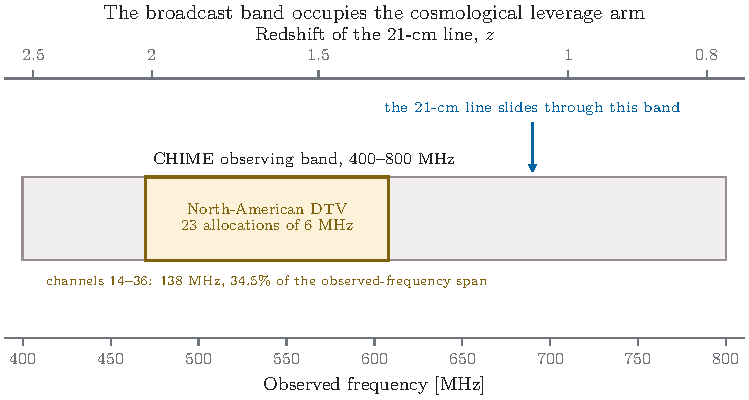
\includegraphics[width=0.98\linewidth]{figs/fig_intro_band.pdf}
\caption{The contested ground. CHIME observes 400--800~MHz; North American digital television occupies 470--608~MHz, which the 21~cm line maps to redshifts $1.34 \le z \le 2.02$ --- a third of the band, sitting on the deepest redshifts CHIME reaches. The 138~MHz of television spectrum is organized as 23 allocations of 6~MHz each (ATSC physical channels 14--36). The figure marks the completed August 2026 coverage: all 23 allocations (channels 14--36, $470$--$608$~MHz) carry archive products and the residual-chain analysis of Chapter~\ref{sec:bao}.}
\label{fig:intro:band}
\end{figure}

Figure~\ref{fig:intro:band} shows the problem in one strip. North American over-the-air television occupies 470--608~MHz, dead center in CHIME's band. For the 21~cm line those frequencies are redshifts 1.34 to 2.02 --- not an incidental corner of the measurement but a third of the band, and the third that reaches deepest into cosmic history. Each television station holds a 6~MHz allocation; twenty-three of them tile the range. There is no moving the telescope away from this: the spectrum is allocated by regulators, the transmitters are licensed to run at high power from elevated sites, and the telescope's own interference surveys identify television bands among the strongest persistent features in its spectrum \cite{amiri2022chime}.

It is worth dispatching the obvious remedies before reaching for a subtle one, because each fails in an instructive way. \emph{Point somewhere else}: a transit telescope has no pointing to change, and the contested frequencies are the science --- there is no elsewhere. \emph{Filter the band out in hardware}: an analog notch per allocation would excise all 138~MHz permanently, which is excision of the very redshifts the measurement wants, purchased in copper instead of software; and a hardware filter cannot be turned off during the hours a transmitter happens to be silent, which Chapter~\ref{sec:bao} will show is where most of the recoverable science lives. \emph{Move the telescope}: it is already in a protected radio-quiet valley, and the television power arrives anyway --- diffracted over the horizon and scattered off aircraft and meteor trails \cite{amiri2022chime}. Distance and terrain attenuate broadcast television; they do not remove it, and this measurement's tolerance is not ``attenuated,'' it is a number. What remains is the subtle remedy: decide, moment by moment and in software, when each channel is contaminated, and discard exactly those moments. The rest of this dissertation is the theory, construction, and pricing of that decision.

Here is the fact that makes this a dissertation rather than a nuisance: \emph{in any single data frame, the television signal is below the telescope's noise.} CHIME integrates in frames of about 42~ms (Section~\ref{sec:system:detector}), and in one frame the measured television power on the channels studied here sits 10 to 35~dB below thermal noise --- between ten and three thousand times weaker (Chapter~\ref{sec:bao}). Nothing about a single frame looks wrong. A sky map made from an afternoon of data would show nothing amiss. If the interference behaved like noise, it would average away with the noise and could be ignored entirely. The whole problem, and the whole of this work, comes from the fact that it does not.

\section{Two Ways to Be Wrong}
\label{sec:intro:errors}

The vocabulary of the problem is worth pinning down, because every quantitative claim in this dissertation is stated in it.

\begin{description}
\item[Statistical error (the error bar).] The scatter a measurement would show if it were repeated many times. It comes from randomness --- here, thermal noise in the receivers --- and it shrinks with more data, as $1/\sqrt{t}$ for observing time $t$. When an experiment quotes $x \pm \sigma$, the $\sigma$ is this.
\item[Systematic.] Anything in the apparatus or environment that pushes the measurement consistently in one direction, rather than randomly in both. A bathroom scale that reads two pounds heavy is a systematic; weighing yourself every morning for a year does not fix it, it just gives you a very precise wrong weight.
\item[Bias.] The shift a systematic produces in the final answer: the distance between the average of many repeated measurements and the truth. Written $b$ throughout.
\item[Residual, $r$.] The unit this dissertation prices contamination in: interference power that survives all filtering into the final statistical analysis, expressed as a fraction of the thermal noise power in the same data (Chapter~\ref{sec:bao}). A residual of $r = 10^{-3}$ means the surviving contamination carries a thousandth of the noise power.
\end{description}

\begin{figure}[t]
\centering
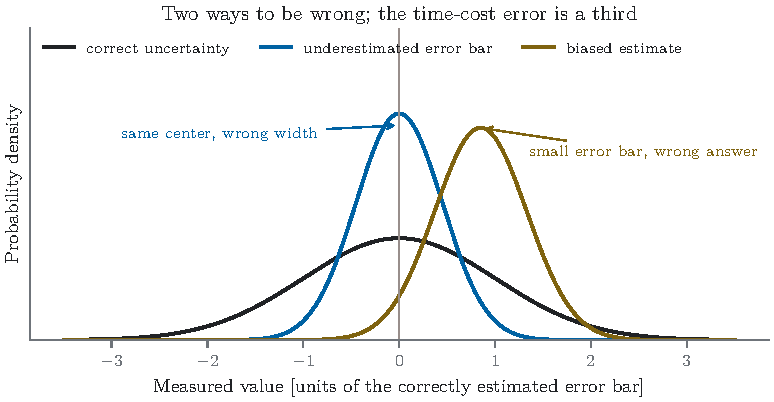
\includegraphics[width=0.98\linewidth]{figs/fig_intro_two_errors.pdf}
\caption{Two ways to be wrong (schematic). Each curve is the distribution of answers an experiment would give if repeated. More data narrows the distribution --- the statistical error falls --- but does nothing to the offset a systematic causes. The same bias that was hidden inside a wide early error bar becomes a confident, precise, wrong answer later: here $b = 0.6$ early error bars, invisible at first, is a $2.4\sigma$ discrepancy after sixteen times the data. The published tolerance criterion, $b \le \sigma$ \cite{amara2008}, is the statement that a measurement should never be allowed into that regime.}
\label{fig:intro:twoerrors}
\end{figure}

Figure~\ref{fig:intro:twoerrors} draws the distinction. Statistical error and bias are not two flavors of the same problem; they respond oppositely to the one resource a survey controls, which is time. Integration narrows the error bar and leaves the bias alone, so the \emph{ratio} of bias to error bar grows as data accumulate. An experiment with an unaddressed systematic does not converge to the truth slowly. It converges, confidently, to the wrong answer --- and every internal consistency check based on scatter will say things are going well.

When is a bias small enough to live with? The convention this work adopts is the one published for precision cosmology by Amara \& R\'efr\'egier \cite{amara2008}: a systematic is tolerable while the bias it induces does not exceed the statistical error, $|b| \le \zeta\,\sigma$ with $\zeta = 1$. The logic is that an experiment's headline number is $x \pm \sigma$; if the truth lies within the quoted interval, the report is honest even in the presence of the systematic. Past that point the experiment is claiming precision it does not have. Nothing about $\zeta = 1$ is magic --- a collaboration wanting margin can set $\zeta = 0.3$ and every tolerance in this work scales linearly --- but $\zeta = 1$ is the published, citable line between an honest error bar and a false one, and Chapter~\ref{sec:bao} adopts it as the definition of ``tolerable.''

\section{Why Time Does Not Fix This One}
\label{sec:intro:coherent}

\begin{figure}[t]
\centering
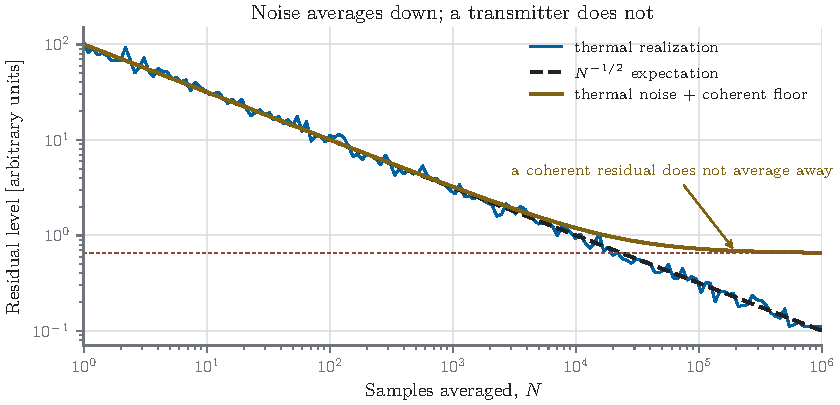
\includegraphics[width=0.98\linewidth]{figs/fig_intro_averaging.pdf}
\caption{One seeded simulation of the mechanism at the heart of the problem. Blue: the running average of pure noise falls as $1/\sqrt{N}$ indefinitely. Orange: add a constant signal at $1/100$ the noise amplitude --- 40~dB weaker in power, invisible in any single sample --- and the average tracks the noise until $N \sim 1/a^2$, then lands on the transmitter and stays there. Averaging is not a filter against something that does not fluctuate. The measured version of this figure, with both axes in survey units, is the convergence analysis of Chapter~\ref{sec:bao}.}
\label{fig:intro:averaging}
\end{figure}

Why doesn't the television signal just average away with the noise it hides beneath? Because averaging removes fluctuations, and a broadcast transmitter, to first approximation, does not fluctuate. Picture a choir of a thousand people each humming a random note that changes every second, and one quiet singer holding a single steady pitch. In any one second the singer is inaudible. Record for an hour and average: the random hums cancel toward silence, and what remains is the held note. The telescope's thermal noise is the choir; the transmitter is the singer.

Figure~\ref{fig:intro:averaging} shows the arithmetic. Noise averages down as $1/\sqrt{N}$ without limit. A coherent signal of amplitude $a$ (in noise units) does not average down at all, so after roughly $N \sim 1/a^2$ samples it owns the average. A signal 40~dB below the noise --- thoroughly undetectable in any frame --- dominates after $10^4$ samples. At the 41.94-ms decision cadence, a continuously integrated channel contributes about $2.06\times10^6$ frames per day. The eight-year forecast target therefore makes even sub-noise coherent residuals dangerous: under the screening model of Chapter~\ref{sec:bao}, contamination that begins 10--35~dB under the noise can exceed the adopted tolerance by factors of roughly three hundred thousand to five hundred thousand if left untreated. Those ratios are forecast outputs, not counts inferred from the sparse trigger archive.

The boundary between ``averages away'' and ``accumulates'' has a name that will recur throughout this work: the \textbf{correlation time}, $\tau_c$ --- how long the contamination holds steady before it changes character. Whatever varies faster than a frame averages down like noise; whatever holds steady accumulates coherently for as long as it holds, and is amplified relative to noise by the number of frames per correlation time. A residual with a 45-minute correlation time is some 64,000 frames' worth more dangerous than its single-frame power suggests, which is why Chapter~\ref{sec:bao} spends considerable effort measuring $\tau_c$ per channel --- and declining to guess where the archive cannot support a measurement.

Reality is gentler than the cartoon in one important way, but the mitigation must be defined at the level where it is applied. The downstream analysis subtracts a per-sidereal-day mean from each \emph{complex visibility}, suppressing contamination that is stationary in sidereal coordinates while retaining the portion that varies within a day through propagation flutter, aircraft reflections, or other changes. The current archive does not contain the corresponding before-and-after visibility products; it contains a scalar pilot-power proxy. In that proxy, the measured intra-day shares span roughly 0.5\%--29\%, equivalent to screening suppressions of about 5--23~dB. These are not direct measurements of complex-visibility attenuation. Chapter~\ref{sec:bao} therefore treats the proxy-to-visibility transfer as an explicit closing test rather than silently crediting the full scalar suppression.

One more twist separates this figure from the real analysis: the time scaling depends on what is held fixed. In the screening calculation of Chapter~\ref{sec:bao}, the residual template is normalized to the survey noise at a declared target time, so the induced bias and statistical error can fall at similar rates and their ratio remains nearly flat. A fixed physical contaminant need not follow that family; as the thermal error shrinks, its significance can instead grow. The dissertation therefore does not infer safety from convergence alone. It defines the residual model, the target observing time, and the tolerance together, and it treats alternative time scalings as a validation gate.

\section{How Much Is Too Much: From a Criterion to a Number}
\label{sec:intro:tolerance}

The criterion $|b| \le \sigma$ is a principle, not a number. Turning it into a number an engineer can design against takes three steps, and the machinery for all three is a \textbf{Fisher forecast}. Fisher information formalizes a simple question: \emph{how sharply do the data distinguish nearby universes?} Imagine generating the map CHIME will measure in two cosmologies that differ only slightly in one parameter --- the bump shifted by a hair. If the two predicted maps differ by much more than the noise, the data carry a lot of information about that parameter; if the difference drowns in noise, they carry little. Fisher information is that ratio, made precise, and its reciprocal square root is the best statistical error any analysis of those data can achieve. A Fisher forecast assembles this for every parameter at once, given an instrument, a sky, and an observing time --- before any data are taken. The forecast used throughout this work is built on the RadioFisher framework of Bull et al.\ \cite{bull2015}, configured to CHIME following its Overview forecast conventions \cite{amiri2022chime}, and it predicts the statistical error $\sigma(\theta)$ on each parameter $\theta \in \{\alpha_\perp, \alpha_\parallel, f\sigma_8\}$ as a function of integration time.

The three steps. First, compute $\sigma(\theta;T_\star)$ for the clean survey at a declared target integration time $T_\star$ --- that is the error bar the experiment is entitled to. Second, inject a small coherent residual with amplitude ratio $r_{\rm sys}$ and compute the first-order shift $\Delta\theta(r_{\rm sys};T_\star)$ it drags into each parameter. Third, solve $|\Delta\theta| = \zeta\,\sigma$ for the allowed residual. The solution,
\[
r_{{\rm sys},\,\rm tol}(\theta;T_\star)
\;=\;
\zeta\,
\frac{\sigma(\theta;T_\star)}
     {\left|\partial\Delta\theta/\partial r_{\rm sys}\right|_{T_\star}},
\]
is the \textbf{tolerance}: the largest residual admitted by that estimator, residual template, and target time before the quoted error bar on $\theta$ becomes misleading. In the current noise-normalized screening family the ratio is nearly flat with integration time, but Chapter~\ref{sec:bao} keeps the target time explicit and requires a separate fixed-physical-amplitude test. For the redshifts occupied by television, the screening tolerances are a few times $10^{-2}$ for the acoustic dilations and $1.5\times10^{-3}$ for $f\sigma_8$: the growth rate is ten to twenty-five times more delicate than the ruler itself, for the position-versus-amplitude reason drawn in Figure~\ref{fig:intro:dilation}.

It is worth being explicit about the three distinct jobs this forecast does in this dissertation, because together they are the reason the cosmological machinery belongs in an instrumentation thesis at all.

\emph{Feasibility.} Before live integration, the forecast asks whether a channel has any defensible operating point under the declared model. The useful comparison is not merely whether a positive tolerance exists, but whether the measured proxy, transfer uncertainty, occupancy, and available suppression can place both stochastic variance and coherent bias inside their gates. The current archive produces conditional recovery candidates on a subset of the ten measured channels, negative screening results on others, and two cases whose outcome is controlled by measurements the snapshot cadence cannot supply. That mixture --- rather than a blanket claim of recoverability --- is why the detector and the decision framework are both needed.

\emph{Evaluation.} In the archival analysis, the same forecast converts measured mask fractions and kept-frame pilot proxies into screening quantities that can be compared with the tolerance, channel by channel. Those comparisons become deployment verdicts only after the proxy is calibrated across each 6-MHz allocation and into visibility-domain residuals, the combined-bin estimator is reproduced, and the per-epoch policies pass blocked holdout tests. Chapter~\ref{sec:bao} carries the present calculation end to end and labels each conclusion by the evidence it actually has.

\emph{Optimization.} Masking is not free. Every flagged frame is discarded observing time, so an aggressive threshold trades residual contamination for a longer survey. For the stochastic part, the equivalent-time cost is $(1+r_{\rm var})/(1-f)$, where $f$ is the masked fraction and $r_{\rm var}$ is the visibility-domain excess-variance ratio. The coherent component $r_{\rm sys}$ is constrained separately by the Fisher-bias tolerance rather than folded into that variance penalty. Pricing the two effects with separate gates turns the threshold from a taste into an optimization variable --- and identifies channels where no tested policy wins.

\section{The Needle in the Shelf}
\label{sec:intro:needle}

\begin{figure}[t]
\centering
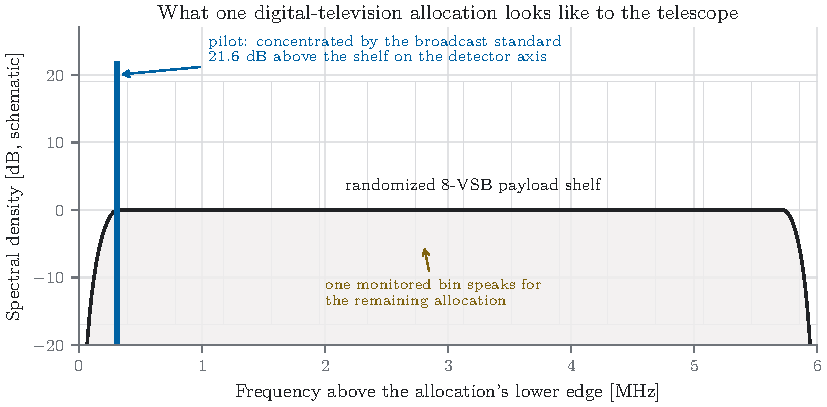
\includegraphics[width=0.98\linewidth]{figs/fig_intro_atsc.pdf}
\caption[One ATSC allocation and its pilot proxy]{What one television allocation looks like to the telescope (schematic, drawn to the measured proportions). The 6~MHz shelf is the broadcast's randomized data payload; in narrow time--frequency cells it can approach the null assumed by power- and variability-based flaggers. The pilot carries about 7\% of the station's power at a nominal standard-defined offset \cite{atsc-a53}: weak in total, but 21.6~dB \emph{above} the shelf in spectral density under the transmitter-ratio model used here. CHIME's 390.625~kHz channel raster is drawn behind; the detector monitors the bin containing the pilot as a proxy for the 15.36 bins spanned by the allocation. Chapters~\ref{sec:dtv} and \ref{sec:param} derive the geometry and state the transfer assumptions.}
\label{fig:intro:atsc}
\end{figure}

CHIME already runs interference flaggers in production, and they work by the natural principle that contamination should look \emph{different} --- an outlier against its neighbors in time, or statistics inconsistent with the adopted noise null (the median-deviation and spectral-kurtosis families; \cite{amiri2023detection,nita2010sk}). Against bursty, above-noise interference that principle is effective. A continuous sub-noise 8-VSB transmission is a harder case: the standard randomizes the payload to flatten its spectrum, and after channelization its narrow-cell statistics can lie close to the same null used by common power and variability tests \cite{atsc-a53}. It need not be mathematically Gaussian, nor is every flagger blind to it; the narrower claim tested here is that the incumbent archive flags are most responsive to transitions while long transmitter-on intervals can remain. The pilot supplies a deterministic feature against which that failure mode can be measured directly.

But the standard, having hidden the payload, could not hide everything. A receiver needs something deterministic to lock onto, so ATSC adds a \textbf{pilot}: a bare carrier at a frequency fixed by the standard to within transmitter tolerance, carrying about 7\% of the station's power \cite{atsc-a53}. Figure~\ref{fig:intro:atsc} shows the anatomy. Seven percent sounds like a poor handle until you notice \emph{where} that power sits: all of it at one known frequency, while the other 93\% is smeared across 6~MHz. In the detector's own analysis bandwidth --- the $3$~kHz bin that detection sensitivity actually responds to --- the pilot stands 21.6~dB \emph{above} the shelf that carries it; per hertz of spectrum the contrast is larger still, about 56~dB (Chapter~\ref{sec:dtv}). The needle is brighter than the haystack, 146-fold, provided you know exactly where to look. And we do know: the broadcast standard is the calibration document.

The detector this dissertation builds is, at its core, one line of mathematics: correlate the data against a copy of what the pilot should be, and compare the power at the pilot's frequency to the power at two reference frequencies a few kilohertz away. That correlation is a matched filter --- a single-term discrete Fourier transform, evaluated off the telescope's frequency grid so it lands exactly on the pilot, implemented as a dot product with precomputed integer weights (Chapter~\ref{sec:param}). Per 42~ms frame, per monitored channel, it yields one number and one decision: transmitter on, or off. Everything else in Chapters~\ref{sec:param}--\ref{sec:impl} --- the weight synthesis, the reference placement, the exact integer arithmetic that makes every implemented decision bit-reproducible --- is engineering in service of that one dot product.

The economics of the method come from a geometric accident shown in the same figure. The pilot occupies one of CHIME's 390.625~kHz bins, but its allocation spans 15.36 of them: one monitored bin speaks for fifteen. Across the whole band, watching 23 pilot bins --- 6.5\% of the contested spectrum --- decides the fate of all 138~MHz. The detector is designed and benchmarked for frame-continuous use, and its decision is per-frame, so a future live mask can remove transmitter-on time rather than entire channels.

\section{What the Detector Must Be}
\label{sec:intro:requirements}

The physics of the preceding subsections is a requirements document in disguise. Collecting the demands in one place shows why the detector of Chapters~\ref{sec:param}--\ref{sec:impl} has the shape it has, and gives the reader a checklist to carry into those sections.

\begin{description}
\item[R1 --- See below the noise.] The contamination sits 10--35~dB under thermal noise per frame, so a detector that inspects raw power is blind by construction. The pilot's 21.6~dB spectral concentration (Chapter~\ref{sec:dtv}) plus coherent integration across each frame (Chapter~\ref{sec:param}) must together close that gap.
\item[R2 --- Decide per frame.] Transmitter occupancy changes on minutes to years, and every misclassified frame either leaks contamination or discards good sky. The decision cadence is one verdict per 42~ms frame per channel (Chapter~\ref{sec:pipeline}), so the mask can remove transmitter-on \emph{time} rather than defaulting to whole-channel excision whenever clean frames remain.
\item[R3 --- Fit the compute budget.] The decision must run on every frame of every contested channel, indefinitely, inside a correlator that is already the busiest part of the instrument. The design therefore reduces the online work to one fixed-point dot-product pipeline per frame (Chapter~\ref{sec:param}) and treats measured runtime, memory traffic, and synchronization headroom as deployment gates rather than assuming the cost is negligible.
\item[R4 --- Reproduce to the bit.] Eight years of archive products are calibrated against this detector's outputs, and the intended live stage uses the same arithmetic contract. Every emitted runtime decision is therefore required to be bit-identical to a reference implementation (Chapter~\ref{sec:impl}): not close, identical, so that any decision can be re-derived and audited years later.
\item[R5 --- Record the statistic, not just the verdict.] The survey products store the full decision statistic for every \emph{processed} frame, not merely the mask bit (Chapter~\ref{sec:pipeline}). This is what lets Chapter~\ref{sec:bao} re-decide every threshold offline, calibrate operating points against the forecast, and adapt to a broadcast environment that measurably changes over the archive --- all without ever re-running the survey.
\end{description}

A sixth demand runs through the analysis rather than the hardware: \emph{prefer ``unmeasured'' to a guess}. Where the archive cannot support a number --- a correlation time on an episodic channel, a sensitivity floor on a channel that never falls quiet --- the machinery of Chapter~\ref{sec:bao} is built to refuse and to carry the refusal forward as a labeled bound, because a budget assembled from optimistic guesses is precisely how a survey ends up confidently wrong, which is the failure mode this entire work exists to prevent.

\section{Limits Within the Mask-and-Discard Paradigm}
\label{sec:intro:optimal}

A masking method invites an obvious objection: perhaps a more sophisticated detector would save channels this one cannot. The right answer is narrower than ``ours is optimal,'' because three distinct questions are easy to conflate: the optimal statistic for a declared signal model, the best complete detector after nuisance parameters and calibration are introduced, and the existence of clean frames for any mask to retain.

\emph{The model-conditional sensitivity result.} For the decision ``is a signal of known form present in Gaussian noise,'' the Neyman--Pearson lemma \cite{neyman1933} establishes that the likelihood-ratio test maximizes detection probability at fixed false-alarm rate, and for a known signal in Gaussian noise that test is the matched filter \cite{north1943,kay1998}. The pilot projection used here is therefore optimal for the known-tone component of the declared model. The complete operational detector is broader: it searches a finite residual-frequency window, estimates local background from displaced references, tolerates feed covariance and non-Gaussian tails through empirical calibration, and applies a rank statistic. Those additions are necessary because the telescope does not satisfy the ideal model exactly, and they prevent the matched-filter theorem from becoming a claim of global optimality for every possible detector.

The broadcast standard also contains deterministic data-segment and data-field synchronization sequences, so the pilot is not literally the only deterministic structure in an 8-VSB waveform \cite{atsc-a53}. It is, however, the dominant \emph{continuously present, spectrally concentrated} feature available to a low-cost detector that does not decode the broadcast. The scrambled payload is noise-like at the time and bandwidth scales used here; the synchronization structures are distributed across the allocation; and the pilot places its coherent energy in one known spectral neighborhood. This is why a pilot matched filter is the natural sensitivity benchmark. It does not prove that every cyclostationary, decoding, multi-antenna, or subtraction method must perform worse. A fair successor comparison would require matched compute, identical frames, and out-of-sample receiver-operating curves.

\emph{The occupancy result.} A different bound applies to channels whose transmitter is effectively always on. If a channel contains no demonstrable clean population, perfect detection within the mask-and-discard paradigm converges to excision: every contaminated frame is rejected and nothing remains. Imperfect detection retains contamination. This conclusion is detector-independent only in that restricted sense. It says that a better \emph{mask} cannot manufacture clean exposure; it does not rule out waveform subtraction, spatial nulling, decoding-assisted cancellation, or a different observing strategy. Chapters~\ref{sec:calibration} and \ref{sec:bao} therefore use ``excision candidate'' rather than ``impossible'' whenever the archive cannot itself establish a clean population.

The boundary is scientifically useful. Sensitivity-limited channels motivate a better detector or a better reference model. Occupancy-pinned channels motivate a different paradigm. The two should not be given the same negative label, and the status matrix in Chapter~\ref{sec:conclusions} keeps them separate.

\section{What This Dissertation Does}
\label{sec:intro:roadmap}

The argument of the work, compressed to a paragraph: CHIME's BAO measurement carries a computable tolerance for surviving contamination, and broadcast television --- sub-noise per frame and potentially coherent across long integration --- can exceed it while evading simple variability-based defenses. The astrophysics leads and the engineering follows: the forecast asks first whether a sufficiently clean mask could make these redshifts useful. The pilot then provides a continuously present, spectrally concentrated target whose projection is a matched filter under the declared model and is cheap enough to evaluate on every processed frame. This dissertation builds that detector to a bit-reproducible engineering contract, applies it to eight years of triggered archival captures, and prices the resulting policies in the currency of the science. The final step is explicitly conditional: a channel verdict is only as strong as the pilot-to-shelf, visibility-domain, and forecast-estimator transfers that connect a detector statistic to cosmology.

The chapters follow that arc. Chapter~\ref{sec:system} sets the instrument and the detection problem. Chapter~\ref{sec:dtv} extracts the pilot from the broadcast standard and establishes every property the detector will rely on. Chapter~\ref{sec:param} synthesizes the matched filter's weights under the telescope's integer arithmetic constraints. Chapter~\ref{sec:pipeline} builds the processing pipeline and its decision theory, and Chapter~\ref{sec:impl} verifies the implementation to the bit. Chapter~\ref{sec:bao} is the reckoning: the residual chain from a masked frame to a cosmological bias, the tolerance derivation sketched above in full, the four-way comparison against keeping everything, excising everything, and the incumbent flaggers, the ten-channel status map, and the August 2026 completion of the thirteen lower-band allocations. Chapter~\ref{sec:deployment} then states the live-stage interface as an engineering contract rather than treating archive execution as telescope deployment, and Chapter~\ref{sec:conclusions} separates measured results, model-conditional forecasts, and the closing tests required before a final 23-channel verdict.

